\subsection{Aplicação Painel - Desativar/Ativar}
\subsubsection*{Descrição do caso de uso}
Desativar um registo significa que este se vai manter na base de dados, mas não irá constar mais nas UI da aplicação de Fábrica. Para \textit{desativar/ativar} um registo, o utilizador necessita pressionar o botão \textit{desativar/ativar} na linha referente ao registo que pretende atualizar. Pelo facto de ser apenas uma procedimento executado em \textit{background}, não possui nenhuma view.

\subsubsection*{\textit{Models} compatíveis com o caso de uso}
Este caso de uso é compatível com os \textit{models} Colaboradores, Pontos de Recolha e Clientes.

\subsubsection*{Fluxo do caso de utilização}
O caso de uso inicia-se quando o utilizador pressionar o botão desativar/ativar da linha do registo que pretende desativar/ativar. Após executar a ação é apresentada uma mensagem ao utilizador, tal como demonstrado na figura \ref{fig:sd_desativar}


\begin{figure}[H] 
	\begin{center}
		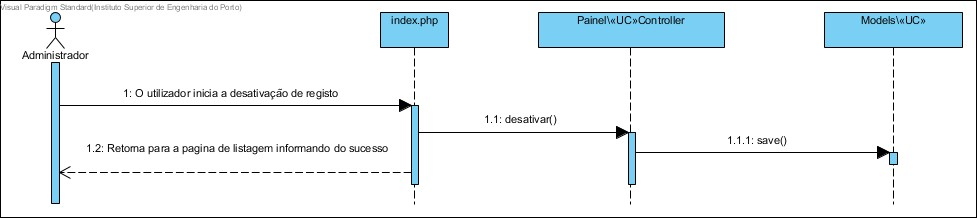
\includegraphics[width=\textwidth,keepaspectratio]{figuras/Diagramas_vp/SD_Painel_5_Desativar.jpg}
		\caption{Diagrama de sequência de desativar/ativar registo}
		\label{fig:sd_desativar} 
	\end{center}
\end{figure}